\documentclass[a4paper,twoside,12pt]{book}

\usepackage[utf8]{inputenc}                                 
\usepackage[T1]{fontenc}  
% ---\usepackage[polish,british]{babel} ---
\usepackage[polish]{babel}
\usepackage{amsmath,amsfonts,amssymb,amsthm}
\usepackage{graphicx,float,subcaption}
\usepackage{mathtools,booktabs,tikz,pgfplots}
\pgfplotsset{compat=1.18}
\usepackage{xurl,csquotes,setspace,indentfirst}
\usepackage{hyperref}
\usepackage{geometry}
\usepackage{fancyhdr}
\usepackage{listings}
\usepackage{adjustbox}


\usepackage[natbib=true,backend=bibtex,maxbibnames=99]{biblatex}
\addbibresource{biblio.bib}

\geometry{margin=2.5cm}
\onehalfspacing
\frenchspacing

\pagestyle{fancy}
\fancyhf{}
\fancyhead[LO]{\nouppercase{\it\rightmark}}
\fancyhead[RE]{\nouppercase{\it\leftmark}}
\fancyhead[LE,RO]{\it\thepage}

\lstset{
    language={[Sharp]C},
    morekeywords={string,exception,std,vector},
    commentstyle=\textit,
    identifierstyle=\textsf,
    keywordstyle=\sffamily\bfseries,
    tabsize=3,
    frame=lines,
    numbers=left,
    numberstyle=\tiny,
    numbersep=5pt,
    breaklines=true,
    escapeinside={@*}{*@}
}

\newcommand{\FirstNameAuthor}{Jakub Zygmunt}
\newcommand{\SurnameAuthor}{\MakeUppercase{Klimczak}}
\newcommand{\IdAuthor}{167314}
\newcommand{\Supervisor}{dr inż. Lesław Pawlaczyk}
\newcommand{\Title}{Candlelight Mod Repo - zmienić potem na faktyczny tytuł}
\newcommand{\Program}{Informatyka}
\newcommand{\Author}{\FirstNameAuthor\space \SurnameAuthor}
\newcommand{\Specialisation}{Zaawansowane systemy baz danych}

\begin{document}
\frontmatter

% --- Title Page ---
\pagestyle{empty}
{\newgeometry{top=1.5cm,bottom=2.5cm,left=3cm,right=2.5cm}
\sffamily
\begin{center}
    
\includegraphics[width=50mm]{figures/layout_set_logo.png}
    
    \vfill
    {\Large\bfseries\Title\par}\vspace{4em}
    {\large\bfseries\Author\par}
    {\normalsize\bfseries Id: \IdAuthor}\vspace{2em}
    
    {\large\bfseries Kierunek:} \Program\\
    {\large\bfseries Specjalizacja:} \Specialisation\vspace{4em}
    
    {\large\bfseries Opiekun}\\
    {\large\Supervisor\par}\vspace{4em}

    \vfill
    
    {\large\bfseries Chorzów, \the\year}
\end{center}

\restoregeometry}

\mainmatter

% --- Spis treści ---

\tableofcontents

% --- Start ---

\chapter{Wprowadzenie}

\section{Przedmowa}

Modyfikacje do gier stają się z biegiem lat standardem branży w sektorze PC. Wiele gier zawdzięcza dużą część swojej widowni właśnie nim. Modyfikacje, potocznie zwane 'mody', są - jak nazwa wskazuje - modyfikacjami kodu gier zazwyczaj stworzonymi przez użytkowników (a nie oryginalnych twórców) w celu zmiany zachowania bądź działania danego programu. Coraz częściej ludzie chcą dzielić się swoimi tworami z innymi pasjonatami. Często jednak ten proces jest bardziej skomplikowany, niż być powinien.

Tematem niniejszej pracy magisterskiej jest odpowiedź na tę potrzebę - aplikacja Candlelight. Jej celem jest stworzenie wygodnego, uporządkowanego i otwartego repozytorium modyfikacji do gier komputerowych. Candlelight umożliwia przeglądanie, ocenianie oraz pobieranie modyfikacji, a także pozwala twórcom publikować nowe wersje i zarządzać nimi. Aplikacja kładzie nacisk na przejrzystość interfejsu, bezpieczeństwo użytkowników oraz skalowalność systemu. System uwzględnia funkcjonalności takie jak mechanizm ulubionych, ocen i recenzji oraz obsługę kont użytkowników, w tym integrację z platformą Steam.

W kolejnych rozdziałach szczegółowo przedstawione zostaną założenia, implementacja oraz możliwości rozwoju tej platformy.

\section{Inspiracja}

Historia modyfikacji do gier sięga nawet jednej z najstarszych gier komputerowych, \textit{Spacewar!}. Była ona wielokrotnie przerabiana oraz rozszerzana przez znajomych autora, Steve'a Russella, którzy zmieniali bądź dodawali jej zawartość \cite{kluska2008}. Scena modyfikacji do gier niezmiernie się od tego czasu zmieniła, coraz szersze grono pasjonatów poświęca wielką ilość czasu na nieodpłatny rozwój swoich ulubionych gier komputerowych. Będąc odbiorcą ich pracy oraz użytkownikiem zarówno modyfikacji jak i wielu stron internetowych im przeznaczonym postanowiłem spróbować swoich sił w ujednoliceniu i zuniwersalizowaniu tego rozproszonego makroświata. 

\section{Cel oraz zakres pracy}

Celem niniejszej pracy jest zaprojektowanie oraz implementacja nowoczesnej aplikacji webowej pełniącej funkcję repozytorium modyfikacji do gier komputerowych. Aplikacja ma umożliwiać użytkownikom przeglądanie, wyszukiwanie, ocenianie oraz publikowanie modów, jak również zarządzanie własnym profilem i ulubionymi pozycjami. Oprócz części funkcjonalnej, istotnym elementem pracy jest także przemyślane zaprojektowanie architektury systemu, w taki sposób, aby był on łatwy w dalszym rozwoju, testowaniu i utrzymaniu.

Zakres pracy obejmuje zarówno backend, jak i frontend aplikacji, wraz z integracją z zewnętrznymi usługami (uwierzytelnianie za pomocą konta Steam), projektowaniem bazy danych oraz wdrożeniem kluczowych mechanizmów umożliwiających publikację i wersjonowanie modów.

W projekcie szczególny nacisk położyłem na stosowanie dobrych praktyk inżynierii oprogramowania oraz podejścia zwinnego (Agile). Dążyłem do tworzenia kodu czytelnego, modularnego, łatwo testowalnego oraz rozszerzalnego w miarę rozwoju wymagań. Starałem się również projektować komponenty w sposób umożliwiający ich ponowne wykorzystanie oraz izolowanie odpowiedzialności (zgodnie z zasadą Single Responsibility Principle), co jest szczególnie istotne przy budowie aplikacji o wielowarstwowej strukturze.

W efekcie, końcowy system nie tylko spełnia założenia funkcjonalne, ale także zgodnie z planem stanowi solidną bazę do dalszego rozwoju, zarówno w kontekście rozbudowy o nowe funkcjonalności przeze mnie lub innych chętnych deweloperów, jak i potencjalnego wdrożenia w środowisku produkcyjnym. Aplikacja stanowi idealną bazę dla osoby chcącej nauczyć się pracy z większym projektem, a z racji open-sourcowej licencji jest ona dostępna do wglądu bądź rozszerzenia dla wszystkich zainteresowanych.

\section{Konkurencyjne rozwiązania}

\chapter{Podstawy teoretyczne wybranych technologii}

W niniejszym rozdziale opiszę używane przeze mnie technologie oraz przyczyny, dla których je wybrałem. Główny stos technologiczny opiera się na rozwiązaniach firmy \textit{Microsoft}, takich jak \textit{ASP.NET Core} oraz \textit{TypeScript}, co pozwoliło na stworzenie nowoczesnej, wydajnej i skalowalnej aplikacji webowej. 

Pomimo dostępności systemu \textit{Microsoft SQL Server}, jako bazę danych zdecydowałem się zastosować \textit{PostgreSQL}, jedno z najpopularniejszych i najlepiej wspieranych rozwiązań open-source w tej kategorii. Wybór ten był podyktowany jego elastycznością, zaawansowanymi możliwościami, pełną kompatybilnością z wykorzystywanym narzędziem \textit{Entity Framework Core} oraz chęcią zaznajomienia się z nim. 

Zamiast technologii \textit{ASP.NET WebForms}, które historycznie związane są ze środowiskiem \textit{Microsoft}, zdecydowałem się na nowoczesne podejście z wykorzystaniem \textit{ASP.NET Core} oraz architektury SPA (Single Page Application) opartej o \textit{Angular}. \textit{WebForms} są uznawane za przestarzałe i niezalecane w przypadku nowych projektów, brakuje im pełnego wsparcia dla współczesnych standardów webowych, komponentów responsywnych oraz rozdzielenia logiki od widoku, co znacząco ogranicza możliwości rozwoju i skalowalności aplikacji. Inną alternatywą \textit{Microsoft}u byłby \textit{Blazor}, ale \textit{Angular} ma dużo lepsze wsparcie 3rd party, a głównym jego atutem jest biblioteka \textit{Angular Material}.

\section{Używane IDE oraz ich rozszerzenia}

Podczas pracy nad projektem używałem dwóch IDE (Integrated Development Environment): \textit{Visual Studio 2022} podczas pracy nad backendem, oraz \textit{Visual Studio Code} podczas pracy nad frontendem oraz do edycji plików konfiguracyjnych i skryptów. Dodatkowo stosowałem \textit{pgAdmin4} \cite{pgadmin2025} do okazjonalnego bezpośredniego skryptowania bazy danych w celach debugowania bądź szybkiego podejrzenia poszczególnych tabel.

\subsection{Visual Studio 2022}

\textit{Visual Studio} jest profesjonalnym zintegrowanym środowiskiem programistycznym powszechnie używanym w branży IT. Zostało stworzone przez firmę \textit{Microsoft}, przez co jest znakomicie przystosowane do pracy nad jej flagową platformą, \textit{.NET}em. \cite{vs2022docs}

Wygodę zwiększa integracja z biblioteką do testów jednostkowych, integracja z \textit{GitHub}em oraz \textit{GitHub Actions}, mechanizmy automatycznego refaktoryzowania kodu, zaawansowany debugger, a także zarządzanie wieloma projektami w ramach rozwiązania. \textit{IntelliSense} wbudowany w środowisko bardzo przyspiesza analizę kodu oraz błędów bez potrzeby kompilacji, pomaga znaleźć miejsca, w których używane są dane zmienne, klasy i metody, a także podpowiada m.in. składowe klas czy argumenty metod. Jest to flagowy produkt \textit{Microsoft}u, co sprawia, że dostaje on częste łatki oraz najwyższej jakości wsparcie. 

Kolejnym atutem jest wbudowany system pakietów \textit{NuGet} \cite{nuget2025}, dzięki któremu można łatwo zarządzać zależnościami projektu, a także \textit{Visual Studio Marketplace} \cite{vsm2025}, które pozwala na wygodne dodawanie rozszerzeń spośród olbrzymiej ilości przygotowanej przez innych developerów. 

Podczas pracy nad projektem korzystałem z rozszerzenia \textit{ReSharper} \cite{resharper2025}, które pozwala przyspieszyć wiele akcji często wykonywanych na kodzie, jak zmiana nazw zmiennych oraz plików, a także informuje o większej ilości błędów oraz problemów niż sam \textit{IntelliSense}.

Drugim wykorzystywanym przeze mnie rozszerzeniem jest \textit{SonarQube}, który pokazuje, jaka część kodu jest pokryta testami, co pomaga zauważyć luki w testach jednostkowych oraz poprawić jakość i niezawodność tworzonego oprogramowania. Do tego pomaga monitorować kod pod kątem potencjalnych błędów, luk bezpieczeństwa czy niezgodności ze standardami \cite{sonarqube2025vs}.

\subsection{Visual Studio Code}

\textit{Visual Studio Code} to lekkie środowisko programistyczne opracowane przez firmę \textit{Microsoft}. W odróżnieniu od \textit{Visual Studio}, jest to edytor kodu z rozszerzalnym ekosystemem, który po odpowiedniej konfiguracji może pełnić funkcję pełnoprawnego IDE. \textit{Visual Studio Code} cechuje się bardzo szybkim działaniem, niskim zużyciem zasobów oraz bogatym zestawem dostępnych rozszerzeń wspierających różne języki i technologie.

Doskonale sprawdza się on zarówno do szybkich edycji plików tekstowych oraz konfiguracyjnych, jak i tworzenia komponentów w \textit{Angular}ze. Dzięki wbudowanemu terminalowi można wygodnie odpalać komendy w trakcie pisania, bez zmiany okna. Wbudowane wsparcie dla systemu \textit{Git} oraz podpowiedzi kodu oparte na mechanizmie \textit{IntelliSense} \cite{vscodeIntellisense2025} sprawiają, że nie odstaje on zbytnio od dużo cięższego konkurenta, \textit{Visual Studio}. 

Wybrałem \textit{Visual Studio Code} do pisania frontendu zamiast pisać wszystko w \textit{Visual Studio} głównie z powodu lepszego wsparcia dla technologii webowych, takich jak \textit{Angular}, SCSS oraz HTML, a także dzięki znacznie lżejszej i bardziej responsywnej pracy edytora przy projektach frontendowych.


\section{PostgreSQL}

\textit{PostgreSQL} to obiektowo-relacyjny system zarządzania bazą danych (ORDBMS), uznawany za jedno z najbardziej zaawansowanych i stabilnych rozwiązań tego typu w świecie open-source. Jest szeroko wykorzystywany zarówno w aplikacjach webowych, jak i systemach analitycznych, dzięki rozbudowanym możliwościom przechowywania danych, obsłudze transakcji ACID, wsparciu dla indeksów złożonych, widoków materializowanych i zapytań zagnieżdżonych \cite{postgresql2025}.

W projekcie \textit{PostgreSQL} służył jako główna baza danych zarówno dla danych użytkowników, jak i przechowywanych danych dotyczących między innymi modów, gier, ocen. Do zarządzania bazą danych i jej strukturą wykorzystywałem migracje \textit{EF Core}, natomiast w przypadkach wymagających ręcznego podejrzenia danych, edycji czy debugowania — posługiwałem się narzędziem \textit{pgAdmin4}.

\textit{PostgreSQL} został wybrany jako system bazodanowy przede wszystkim dlatego, że należy do najpopularniejszych technologii tego typu, co w świecie IT przekłada się na długowieczność projektu, lepsze wsparcie i dużą dostępność zasobów edukacyjnych. Jego pełna zgodność z \textit{Entity Framework Core} dzięki stabilnemu i rozwijanemu providerowi \textit{Npgsql} \cite{npgsql2025} pozwoliła na płynną integrację z backendem opartym o \textit{.NET 8}. \textit{PostgreSQL} oferuje również wsparcie dla zaawansowanych typów danych, takich jak \textit{uuid} czy tablice, które okazały się przydatne przy modelowaniu struktur takich jak listy wersji, zależności czy metadane modów. Istotnym czynnikiem była także wysoka wydajność zapytań — nawet przy pracy z dużymi kolekcjami danych, jak np. statystyki pobrań, oceny czy liczby ulubionych modyfikacji.

\section{.NET oraz Entity Framework}

Platforma \textit{.NET} wraz z \textit{Entity Framework Core} została wybrana ze względu na swoją popularność, stabilność oraz bardzo dobrą integrację z ekosystemem narzędzi firmy \textit{Microsoft}. Umożliwia szybkie tworzenie nowoczesnych, wielowarstwowych aplikacji webowych, jednocześnie oferując wysoką wydajność oraz bezpieczeństwo. Z kolei \textit{Entity Framework Core} pozwala znacząco przyspieszyć rozwój aplikacji dzięki eliminacji potrzeby pisania dużej ilości zapytań SQL oraz automatycznemu odwzorowaniu struktury bazy danych na modele domenowe. Obie technologie są również intensywnie rozwijane, posiadają długoterminowe wsparcie oraz bogatą dokumentację, co czyni je bezpiecznym i przyszłościowym wyborem dla projektu tej skali.

\subsection{.NET 8}
\textit{.NET 8} to najnowsza w momencie rozpoczęcia pracy wersja wieloplatformowej platformy programistycznej firmy Microsoft, wydana w ramach modelu Long-Term Support (LTS). Wprowadza szereg usprawnień wydajnościowych, rozszerzeń językowych oraz ulepszeń związanych z AOT (Ahead-of-Time Compilation), które pozwalają między innymi na szybsze uruchamianie aplikacji i mniejsze zużycie pamięci. Wersja ta pozwala na wykorzystanie nowości języka \textit{C\#} 12, takich jak kolejne usprawnienia składni \textit{primary constructors} czy rozszerzenia \textit{using static}. Dodatkowo, \textit{.NET 8} oferuje uproszczony model konfiguracji aplikacji, rozszerzone wsparcie dla \textit{minimal APIs} oraz usprawnienia w zakresie testowania i obserwowalności aplikacji (między innymi wbudowane OpenTelemetry) \cite{dotnet8overview2025} \cite{dotnet8runtime2025}. Dzięki tym możliwościom, aplikacja mogła być rozwijana zgodnie z nowoczesnymi praktykami i była przygotowana na przyszłościową skalowalność.

W projekcie platforma \textit{.NET 8} została wykorzystana do implementacji warstwy backendowej - REST API, uwierzytelnienia, logiki biznesowej oraz integracji z bazą danych.

\subsection{EF Core 8 oraz Npgsql}

\textit{Entity Framework Core 8} (\textit{EF Core 8}) to obiektowo-relacyjny mapper (ORM) opracowany przez firmę {Microsoft}, służący do pracy z bazą danych w sposób deklaratywny; poprzez definiowanie modeli danych i ich relacji w postaci klas \textit{C\#}. \textit{EF Core} pozwala generować i zarządzać strukturą bazy danych poprzez migracje, co znacząco przyspiesza rozwój aplikacji i ułatwia zachowanie spójności danych \cite{ef2025}.

W projekcie \textit{EF Core} pełnił kluczową rolę w warstwie dostępu do danych, zapewniając wydajne i typowane zapytania \textit{LINQ} oraz automatyczne śledzenie zmian w encjach \cite{ef2025}. \textit{LINQ} (Language Integrated Query) umożliwia tworzenie zapytań bazodanowych w sposób zintegrowany z językiem \textit{C\#}, dzięki czemu można pisać zapytania z pełnym wsparciem IntelliSense, refaktoryzacji i kontroli typów. Takie podejście nie tylko zwiększa czytelność kodu, ale także zmniejsza ryzyko błędów składniowych typowych dla zapytań SQL pisanych ręcznie \cite{linq2025pl}. Dzięki integracji z dostawcą \textit{Npgsql} możliwa była pełna zgodność z \textit{PostgreSQL}, w tym wsparcie dla typów specyficznych jak \textit{uuid} \cite{npgsql2025}.

Biblioteka ta pozwalała również korzystać z rozszerzeń \textit{PostgreSQL} takich jak ILIKE, pełnotekstowe wyszukiwanie oraz funkcje agregujące. Konfiguracja \textit{Fluent API} oraz atrybuty w modelach umożliwiały precyzyjne dostosowanie struktury bazy, a jednocześnie zachowanie przejrzystego kodu w warstwie logiki aplikacji.

\section{Biblioteki backendowe}

\subsection{SpaProxy}
W projekcie zastosowałem \textit{SpaProxy}, który działa jako pośrednik przekazujący żądania HTTP z backendu (hostowanego na porcie, na przykład w przypadku lokalnej konfiguracji Candlelight \texttt{https://localhost:7275}) do serwera deweloperskiego Angulara (na przykład w przypadku lokalnej konfiguracji Candlelight \texttt{http://localhost:4200}). Umożliwia to lokalne uruchamianie aplikacji frontendowej z pełnym wsparciem hot-reload, jednocześnie pozwalając backendowi zachować kontrolę nad routingiem i autoryzacją \cite{aspnetspaproxy2025}.

Zastosowanie \textit{SpaProxy} znacząco usprawniło i przyspieszyło pracę deweloperską - nie było konieczne ręczne kopiowanie plików builda frontendu do katalogu \texttt{wwwroot} oraz możliwa była równoległa praca nad logiką serwera i interfejsem użytkownika. Proxy to jest transparentne w działaniu i eliminuje problemy związane z CORSem podczas lokalnego rozwoju \cite{spaproxy2025}.

\subsection{Steam OpenID}
W celu uwierzytelniania użytkowników za pomocą platformy Steam wykorzystałem protokół \textit{OpenID} w implementacji biblioteki \texttt{AspNet.Security.OpenId.Steam} \cite{steamopenid2025}. Pozwala ona na łatwe zintegrowanie logowania kontem Steam, co w kontekście repozytorium modów gier stanowi bardzo intuicyjne i wygodne rozwiązanie dla użytkowników końcowych.

Biblioteka ta obsługuje cały proces przekierowania do Steam, autoryzacji użytkownika oraz zwrócenia unikalnego identyfikatora konta Steam (SteamID), który może być dalej przechowywany w bazie danych i kojarzony z kontem w aplikacji. Była ona więc idealnym dopasowaniem do moich potrzeb.

\section{Typescript i Angular}

\subsection{TypeScript}

\textit{TypeScript} to nadzbiór języka \textit{JavaScript} rozwijany przez firmę \textit{Microsoft}, który wprowadza statyczne typowanie oraz szereg nowoczesnych funkcjonalności znanych z języków takich jak \textit{C\#} czy \textit{Java}. Dzięki typom, interfejsom i klasom kod jest łatwiejszy do zrozumienia, utrzymania oraz testowania. Pozwala także wykrywać błędy na etapie kompilacji, zanim jeszcze trafią one do przeglądarki.

W kontekście projektu, \textit{TypeScript} znacząco usprawnił implementację komponentów, serwisów oraz modeli danych w \textit{Angularze}, zapewniając przejrzystość i solidność kodu. Użycie interfejsów do reprezentowania struktur danych takich jak gry, modyfikacje czy użytkownicy umożliwiło wygodną integrację z backendem opartym na \textit{.NET}. Dodatkowo, wykorzystanie konstrukcji takich jak \texttt{readonly} podniosło jakość kodu oraz zredukowało potencjalne błędy w trakcie przyszłej pracy zespołowej\cite{typescript2025}.

\subsection{Angular}

\textit{Angular} to jedno z najpopularniejszych frameworków frontendowych, rozwijany przez zespół \textit{Google}. Jest to rozwiązanie typu SPA (Single Page Application), umożliwiające budowę wydajnych, modularnych i łatwo testowalnych aplikacji webowych. \textit{Angular} opiera się na architekturze komponentowej, co znacznie ułatwia zarządzanie złożonym interfejsem użytkownika.

W projekcie używałem \textit{Angular}a do stworzenia interfejsu użytkownika, który umożliwia przeglądanie gier, modyfikacji, logowanie się przez Steam, edycję profilu, a także zarządzanie swoimi ulubionymi modami. Skorzystałem między innymi z takich funkcjonalności frameworka jak:

    \textbf{Angular Routing} do implementacji nawigacji pomiędzy widokami.

    \textbf{Reactive Forms} do obsługi formularzy edycji profilu oraz przesyłania modyfikacji.

    \textbf{HTTPClient} do komunikacji z backendowym REST API.

    \textbf{Dependency Injection} pozwalający na modularne i testowalne serwisy.

\textit{Angular} w wersji 18 zaoferował dodatkowe usprawnienia pod kątem wydajności i lazy-loadingu, oraz był najnowszą stabilną (LTS) wersją w momencie rozpoczęcia prac nad projektem \cite{angular2025}.

\section{Znaczące biblioteki frontendowe}

\subsection{RxJS}

\textit{RxJS} (Reactive Extensions for \textit{JavaScript}) to biblioteka programowania reaktywnego używana w \textit{Angular}ze do pracy ze strumieniami danych i zdarzeń asynchronicznych. Dzięki niej możliwe jest zarządzanie przepływem danych w sposób deklaratywny, z wykorzystaniem operatorów takich jak \texttt{map}, \texttt{filter}, \texttt{switchMap}, \texttt{debounceTime} czy \texttt{combineLatest} \cite{rxjs2025}.

W projekcie \textit{RxJS} był niezwykle przydatnym narzędziem w takich miejscach jak filtrowanie i wyszukiwanie modów/gier, debounceowanie inputów formularzy oraz subskrypcje danych z API. Dzięki asynchronicznemu podejściu można było znacząco uprościć kod komponentów i uniknąć tak zwanego \textit{callback hell} (zagnieżdżone funkcje zwrotne tworzą trudny do odczytania i utrzymania kod).

\subsection{Angular Material}

\textit{Angular Material} to oficjalna implementacja \textit{Material Design} dla \textit{Angular}a. Oferuje zestaw gotowych komponentów UI zgodnych z wytycznymi \textit{Google}, takich jak przyciski, formularze, karty, okna dialogowe, listy, paginatory czy elementy nawigacyjne \cite{angularmaterial2025}. W projekcie wykorzystałem \textit{Angular Material} do stworzenia nowoczesnego i spójnego interfejsu użytkownika. Kluczowe komponenty to:

    \texttt{MatCard} do prezentacji gier i modów w formie kafelków,

    \texttt{MatFormField}, \texttt{MatInput}, \texttt{MatSelect}, \texttt{MatSlideToggle} do obsługi formularzy,

    \texttt{MatPaginator} do implementacji paginacji modów i gier,

    \texttt{MatSnackBar} do pokazywania komunikatów użytkownikowi,

Zaletą \textit{Angular Material} jest responsywność komponentów oraz ich dobra integracja z tematami kolorystycznymi, co pozwoliło mi na spójny i wygodny UI.

\section{Linting kodu i zapobieganie code smellowi}

\subsection{GitHub Actions}

\subsection{ESLint}

\subsection{Prettier}

\subsection{ReSharper}

\subsection{SonarQube}

\section{Biblioteki testowe}

\subsection{Karma Jasmine}

\subsection{NUnit}

\subsection{Moq}

\subsection{Coverlet}

\chapter{Architektura projektu}

\begin{center}
  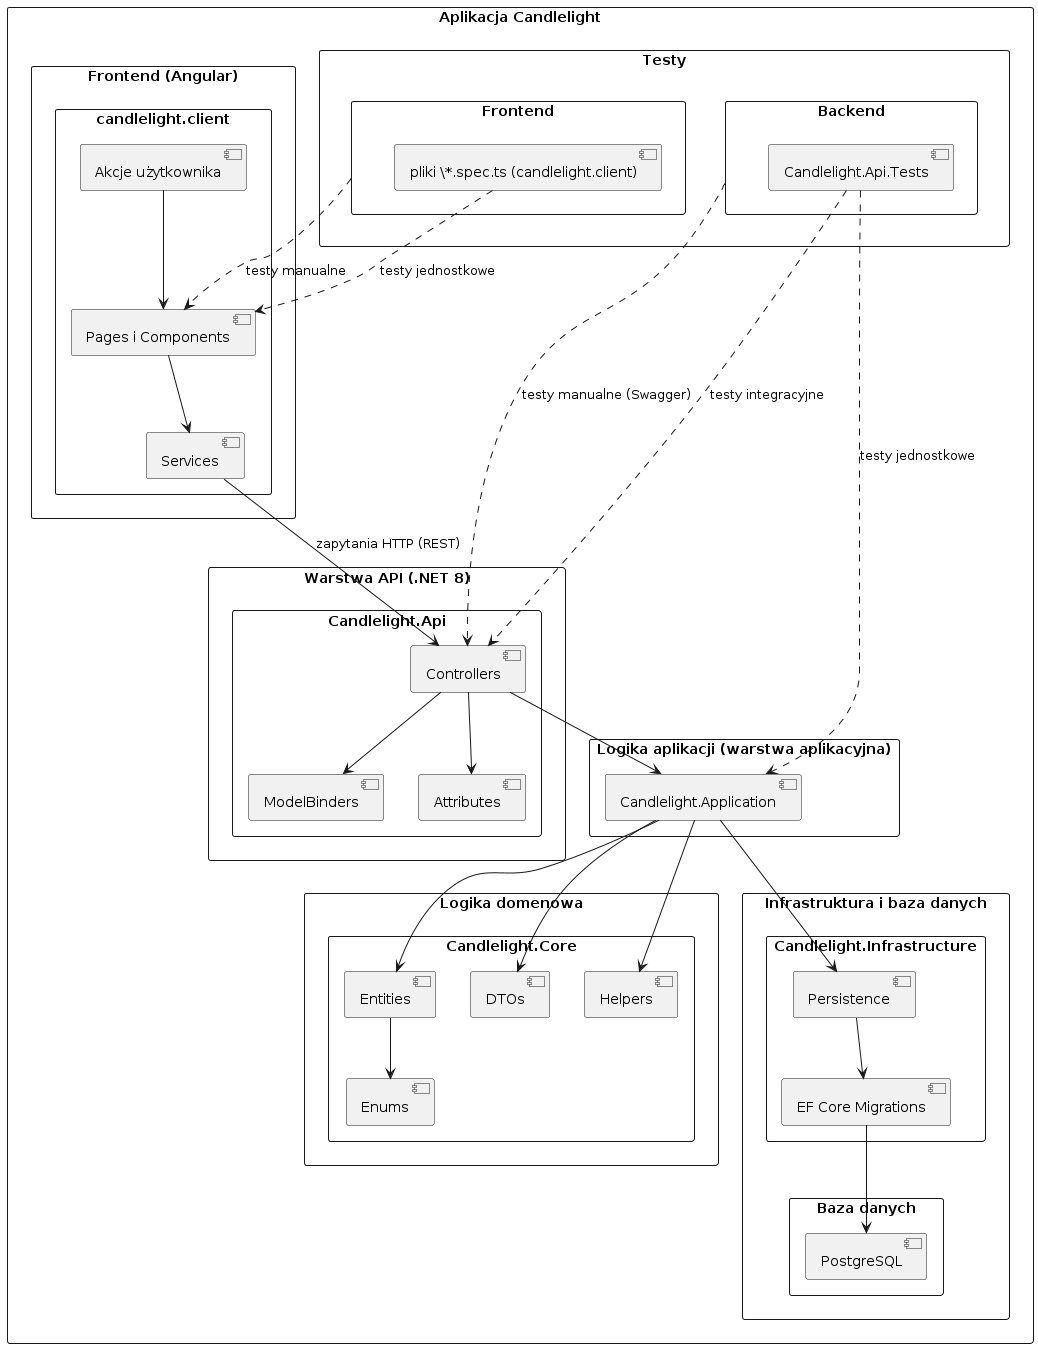
\includegraphics[width=\textwidth, height=0.70\textheight, keepaspectratio]{figures/app-structure.png}  
\end{center}

Struktura projektu została zaprojektowana w duchu architektury wielowarstwowej, umożliwiającej jasny podział odpowiedzialności oraz łatwą skalowalność i utrzymanie kodu. Poniżej przedstawiono główne warstwy i komponenty systemu.


\subsubsection{Struktura warstwy API}
Projekt \texttt{Candlelight.Api} odpowiada za obsługę zapytań HTTP, pełniąc rolę kontrolera dostępowego do logiki aplikacji. Znajdują się tu kontrolery (\texttt{Controllers}), atrybuty do walidacji (\texttt{Attributes}), customowe \texttt{ModelBinders} i pliki statyczne w katalogu \texttt{wwwroot}.

\subsubsection{Struktura warstwy aplikacyjnej}
Projekt \texttt{Candlelight.Application} zawiera logikę biznesową aplikacji. Moduł \texttt{Services} zawiera serwisy odpowiadające za operacje na grach, modach i użytkownikach. Jest to warstwa pośrednia między API a infrastrukturą.

\subsubsection{Warstwa dostępu do danych}
Projekt \texttt{Candlelight.Infrastructure} zawiera implementację dostępu do danych. W katalogu \texttt{Persistence/Data} zdefiniowano kontekst bazy danych oraz konfiguracje encji. Folder \texttt{Migrations} przechowuje migracje bazy danych generowane przez EF Core 8. Wykorzystywany jest provider \texttt{Npgsql} umożliwiający współpracę z PostgreSQL.

\subsubsection{Warstwa domenowa}
Projekt \texttt{Candlelight.Core} gromadzi definicje encji domenowych (\texttt{Entities}), transferowych (\texttt{Dtos}), typów wyliczeniowych (\texttt{Enums}) oraz pomocnicze klasy narzędziowe (\texttt{Helpers}). Stanowi centralny punkt współdzielony pomiędzy pozostałymi warstwami aplikacji.

\subsubsection{Frontend}
Frontend znajduje się w katalogu \texttt{candlelight.client} i został zbudowany przy użyciu frameworka \textit{Angular 18}. Główna logika podzielona została na moduły odpowiadające poszczególnym funkcjonalnościom, główne z nich to:

\begin{itemize}
\item \textbf{auth}: logowanie, rejestracja, Steam login,
\item \textbf{games}: lista gier, szczegóły gry, dodawanie gier,
\item \textbf{mods}: przeglądanie, szczegóły, dodawanie modów,
\item \textbf{user-profile}: profil użytkownika, edycja, ulubione gry i mody,
\item \textbf{shared}: komponenty wielokrotnego użytku (np. paginator, filtry, guardy),
\item \textbf{public}: zasoby statyczne takie jak \texttt{assets} i \texttt{icons}.
\end{itemize}

Struktura ta wspiera modularność oraz umożliwia łatwe dodawanie nowych komponentów.

\subsubsection{Testy jednostkowe}
Projekt \texttt{Candlelight.Api.Tests} zawiera testy jednostkowe dla backendu. Testy te wykorzystują frameworki \texttt{xUnit} i \texttt{Moq}, umożliwiając weryfikację poprawności działania serwisów i kontrolerów w izolacji. Dodatkowo podczas pracy nad kodem wykonywałem regularne testy manualne (często przy użycia \textit{Swagger}a).

Frontend (\textit{candlelight.client}) korzysta z biblioteki do testów jednostkowych Karma Jasmine. Testy te są zawarte w plikach *.spec.ts i są wydzielone na poszczególne komponenty \textit{Angular}owe.

\subsubsection{Zarządzanie konfiguracją i CI/CD}
Folder \texttt{.github/workflows} zawiera konfiguracje GitHub Actions, które odpowiadają za automatyzację procesu budowania, testowania i wdrażania aplikacji. Dzięki integracji CI/CD (\textit{Continuous Integration / Continuous Deployment}) możliwe jest szybkie wychwytywanie błędów i zapewnienie spójnej jakości kodu.

\subsubsection{Zasoby statyczne backendu}
W katalogu \texttt{wwwroot} znajdują się zasoby statyczne służące do przechowywania przesyłanych przez użytkowników plików, takich jak awatary, okładki gier i obrazy modów. Pliki są porządkowane w foldery zgodnie z identyfikatorami encji, co ułatwia zarządzanie oraz zapewnia unikalność nazw.

\chapter{Implementacja funkcjonalności aplikacji}

\section{Obsługa autoryzacji użytkownika}

\section{Zarządzanie profilem użytkownika}

\section{Funkcjonalności związane z grami}

\section{Funkcjonalności związane z modyfikacjami}

\subsection{Przesyłanie modyfikacji oraz ich wersji}

\subsection{Lista modyfikacji dla gry}

\section{Strona główna oraz UX aplikacji}

\section{Integracje z zewnętrznymi serwisami}

\chapter{Podsumowanie projektu}

\section{Trudności i wyzwania}

\section{Wnioski z projektu}

\section{Potencjalne kierunki rozwoju projektu}
...
wydzielenie mikroserwisów komunikujących się przy użyciu Kafki oraz konteneryzacja, integracja z VirusTotal, QoL features, UX work, hosting
...

% --- Bibliografia ---
\cleardoublepage
\phantomsection
\addcontentsline{toc}{chapter}{Bibliografia}
\printbibliography
\end{document}
